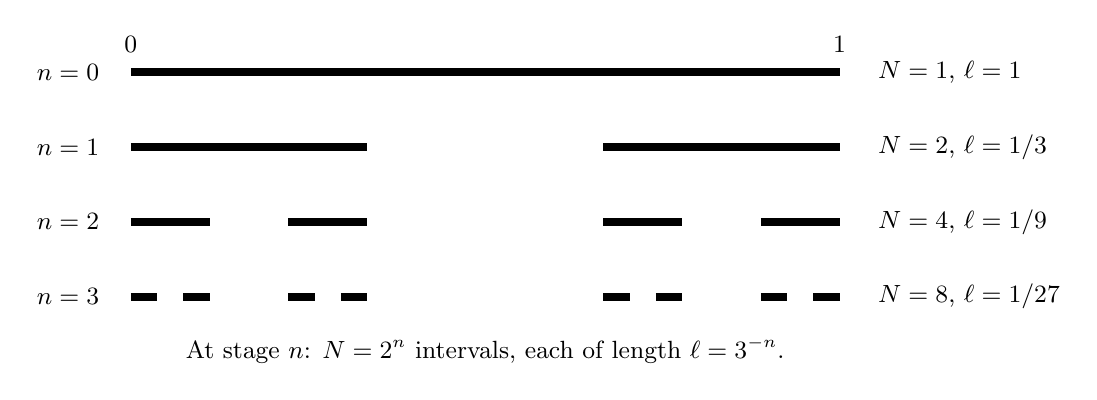
\begin{tikzpicture}[x=9cm,y=0.95cm,font=\small,line width=0.8pt]
  \foreach \stage in {0,1,2,3} {
    \node[left] at (-0.03,-\stage) {$n=\stage$};
  }
  \draw[line width=3pt] (0,0)--(1,0);
  \foreach \numerator in {0,2} {
    \draw[line width=3pt] ({\numerator/3},-1)--({(\numerator+1)/3},-1);
  }
  \foreach \numerator in {0,2,6,8} {
    \draw[line width=3pt] ({\numerator/9},-2)--({(\numerator+1)/9},-2);
  }
  \foreach \numerator in {0,2,6,8,18,20,24,26} {
    \draw[line width=3pt] ({\numerator/27},-3)--({(\numerator+1)/27},-3);
  }
  \node[above] at (0,0.12) {$0$};
  \node[above] at (1,0.12) {$1$};
  \node[right] at (1.04,0) {$N=1$, $\ell=1$};
  \node[right] at (1.04,-1) {$N=2$, $\ell=1/3$};
  \node[right] at (1.04,-2) {$N=4$, $\ell=1/9$};
  \node[right] at (1.04,-3) {$N=8$, $\ell=1/27$};
  \node[below] at (0.5,-3.4) {At stage $n$: $N=2^n$ intervals, each of length $\ell=3^{-n}$.};
\end{tikzpicture}
